\documentclass[12pt]{article}\usepackage[]{graphicx}\usepackage[]{color}
%% maxwidth is the original width if it is less than linewidth
%% otherwise use linewidth (to make sure the graphics do not exceed the margin)
\makeatletter
\def\maxwidth{ %
  \ifdim\Gin@nat@width>\linewidth
    \linewidth
  \else
    \Gin@nat@width
  \fi
}
\makeatother

\definecolor{fgcolor}{rgb}{0.345, 0.345, 0.345}
\newcommand{\hlnum}[1]{\textcolor[rgb]{0.686,0.059,0.569}{#1}}%
\newcommand{\hlstr}[1]{\textcolor[rgb]{0.192,0.494,0.8}{#1}}%
\newcommand{\hlcom}[1]{\textcolor[rgb]{0.678,0.584,0.686}{\textit{#1}}}%
\newcommand{\hlopt}[1]{\textcolor[rgb]{0,0,0}{#1}}%
\newcommand{\hlstd}[1]{\textcolor[rgb]{0.345,0.345,0.345}{#1}}%
\newcommand{\hlkwa}[1]{\textcolor[rgb]{0.161,0.373,0.58}{\textbf{#1}}}%
\newcommand{\hlkwb}[1]{\textcolor[rgb]{0.69,0.353,0.396}{#1}}%
\newcommand{\hlkwc}[1]{\textcolor[rgb]{0.333,0.667,0.333}{#1}}%
\newcommand{\hlkwd}[1]{\textcolor[rgb]{0.737,0.353,0.396}{\textbf{#1}}}%

\usepackage{framed}
\makeatletter
\newenvironment{kframe}{%
 \def\at@end@of@kframe{}%
 \ifinner\ifhmode%
  \def\at@end@of@kframe{\end{minipage}}%
  \begin{minipage}{\columnwidth}%
 \fi\fi%
 \def\FrameCommand##1{\hskip\@totalleftmargin \hskip-\fboxsep
 \colorbox{shadecolor}{##1}\hskip-\fboxsep
     % There is no \\@totalrightmargin, so:
     \hskip-\linewidth \hskip-\@totalleftmargin \hskip\columnwidth}%
 \MakeFramed {\advance\hsize-\width
   \@totalleftmargin\z@ \linewidth\hsize
   \@setminipage}}%
 {\par\unskip\endMakeFramed%
 \at@end@of@kframe}
\makeatother

\definecolor{shadecolor}{rgb}{.97, .97, .97}
\definecolor{messagecolor}{rgb}{0, 0, 0}
\definecolor{warningcolor}{rgb}{1, 0, 1}
\definecolor{errorcolor}{rgb}{1, 0, 0}
\newenvironment{knitrout}{}{} % an empty environment to be redefined in TeX

\usepackage{alltt}
\usepackage{amsmath}
\usepackage{amssymb}
\usepackage{graphicx}
\usepackage{fullpage}
\usepackage{setspace}
\usepackage{hyperref}
\usepackage{color}
\onehalfspacing
\IfFileExists{upquote.sty}{\usepackage{upquote}}{}
\begin{document}

\title{Pol Sci 630: Problem Set 5 - Regression Model Interpretation - Solutions}

\author{Prepared by: Jan Vogler (\href{mailto:jan.vogler@duke.edu}{jan.vogler@duke.edu})}

\date{Grading Due Date: Friday, October 2nd, 12.15 PM (Beginning of Lab)}
 
\maketitle



\textbf{\color{red} Insert your comments on the assignment that you are grading above the solution in bold and red text. For example write: "GRADER COMMENT: everything is correct! - 4/4 Points" Also briefly point out which, if any, problems were not solved correctly and what the mistake was.}

\bigskip

\textbf{Use the following scheme to assign points: For problems that were solved correctly in their entirety, assign the full point value of four. For correctly solved bonus problems, add that value to the total score for a problem but do not go above 4 points per problem. If there are mistakes in any problem, subtract points according to the extent of the mistake. If you subtract points, explain why.}

\bigskip

\textbf{In order to make your text bold and red, you need to insert the following line at the beginning of the document:}

\begin{verbatim} \usepackage{color} \end{verbatim}

\textbf{and the following lines above the solution of the specific task:}

\begin{verbatim} \textbf{\color{red} GRADER COMMENT: everything is correct! - 4/4 Points} \end{verbatim}



\pagebreak

\section*{R Programming}

\subsection*{Problem 1}

\begin{knitrout}
\definecolor{shadecolor}{rgb}{0.969, 0.969, 0.969}\color{fgcolor}\begin{kframe}
\begin{alltt}
\hlcom{### a}

\hlkwd{data}\hlstd{(swiss)}
\hlkwd{summary}\hlstd{(swiss)}
\end{alltt}
\begin{verbatim}
##    Fertility      Agriculture     Examination      Education    
##  Min.   :35.00   Min.   : 1.20   Min.   : 3.00   Min.   : 1.00  
##  1st Qu.:64.70   1st Qu.:35.90   1st Qu.:12.00   1st Qu.: 6.00  
##  Median :70.40   Median :54.10   Median :16.00   Median : 8.00  
##  Mean   :70.14   Mean   :50.66   Mean   :16.49   Mean   :10.98  
##  3rd Qu.:78.45   3rd Qu.:67.65   3rd Qu.:22.00   3rd Qu.:12.00  
##  Max.   :92.50   Max.   :89.70   Max.   :37.00   Max.   :53.00  
##     Catholic       Infant.Mortality
##  Min.   :  2.150   Min.   :10.80   
##  1st Qu.:  5.195   1st Qu.:18.15   
##  Median : 15.140   Median :20.00   
##  Mean   : 41.144   Mean   :19.94   
##  3rd Qu.: 93.125   3rd Qu.:21.70   
##  Max.   :100.000   Max.   :26.60
\end{verbatim}
\begin{alltt}
\hlcom{### b}

\hlstd{lm1} \hlkwb{=} \hlkwd{lm}\hlstd{(Education} \hlopt{~} \hlstd{Fertility} \hlopt{+} \hlstd{Agriculture} \hlopt{+} \hlstd{Examination} \hlopt{+} \hlstd{Catholic} \hlopt{+} \hlstd{Infant.Mortality,}
    \hlkwc{data} \hlstd{= swiss)}

\hlkwd{summary}\hlstd{(lm1)}
\end{alltt}
\begin{verbatim}
## 
## Call:
## lm(formula = Education ~ Fertility + Agriculture + Examination + 
##     Catholic + Infant.Mortality, data = swiss)
## 
## Residuals:
##      Min       1Q   Median       3Q      Max 
## -11.3949  -2.3716  -0.2856   2.8108  11.2985 
## 
## Coefficients:
##                  Estimate Std. Error t value Pr(>|t|)    
## (Intercept)      32.74414    8.87888   3.688 0.000657 ***
## Fertility        -0.40851    0.08585  -4.758 2.43e-05 ***
## Agriculture      -0.16242    0.04488  -3.619 0.000804 ***
## Examination       0.41980    0.16339   2.569 0.013922 *  
## Catholic          0.10023    0.02150   4.663 3.29e-05 ***
## Infant.Mortality  0.20408    0.28390   0.719 0.476305    
## ---
## Signif. codes:  0 '***' 0.001 '**' 0.01 '*' 0.05 '.' 0.1 ' ' 1
## 
## Residual standard error: 4.907 on 41 degrees of freedom
## Multiple R-squared:  0.7678,	Adjusted R-squared:  0.7395 
## F-statistic: 27.12 on 5 and 41 DF,  p-value: 5.223e-12
\end{verbatim}
\end{kframe}
\end{knitrout}

\subparagraph{c)} In order to get full points on this problem, you need an interpretation for each of the 5 variables.

The interpretation would look like this for \textit{Fertility}:

There is a negative linear relationship between \textit{Fertility} and \textit{Education}. For a 1-point increase in Fertility, we expect a 0.41-point decrease in Education, holding all other variables constant. The t-value is -4.758. This t-value implies a p-value of $2.43*10^{-5}$. This $p < 0.001$ corresponds to a type-1 error rate of $\alpha < 0.001$, meaning that the statistical relationship is significant at all common levels of statistical significance.

The other variables are interpreted accordingly. \textit{Agriculture} and \textit{Catholic} are significant at all common levels of statistical significance as well. Please note that \textit{Examination} is significant at a level of $p < 0.05$ ($\alpha < 0.05$) and \textit{Infant.Mortality} is not significant at common levels of statistical significance.

The $R^2$ statistic shows us that our model explains 76.78 percent (multiple $R^2$) or 73.95 percent (adjusted $R^2$) of the variation in the dependent variable --- depending on whether one is penalized for introducing further variables into the model.

The F-statistic shows us that the joint statistical significance of all variables in our model when predicting levels of Education is high. With a p-value of $p < 0.001$, our model estimates a relationship that is significant at all common levels of statistical significance.



\subsection*{Problem 3}

\paragraph{a)} In this task you have to formulate a hypothesis regarding the relationship of several political and economic factors and the level of FDI inflows. For example, you could claim that economic crises generally lead to a lower inflow of foreign investment because countries that experience crises are less attractive to investors.

In a well-known paper in \textit{International Organization}, Nathan Jensen made the claim that democratic institutions can make more credible commitments to upholding property rights, which means that foreign investors trust democratic governments more than authoritarian governments. This implies that countries with democratic political systems should experience more FDI inflows that countries with authoritarian political systems. Regardless of which variable you choose, your hypothesis should look similar to this one:

Hypothesis: Countries with higher levels of democracy experience more foreign direct investment (as percentage of GDP) than countries with lower levels of democracy.

\begin{knitrout}
\definecolor{shadecolor}{rgb}{0.969, 0.969, 0.969}\color{fgcolor}\begin{kframe}
\begin{alltt}
\hlcom{### b}
\hlkwd{library}\hlstd{(foreign)}
\hlstd{LDC} \hlkwb{=} \hlkwd{read.dta}\hlstd{(}\hlstr{"LDC_IO_replication.dta"}\hlstd{)}

\hlstd{lm_fdi} \hlkwb{=} \hlkwd{lm}\hlstd{(fdignp} \hlopt{~} \hlstd{l1polity} \hlopt{+} \hlstd{l1signed} \hlopt{+} \hlstd{l1office} \hlopt{+} \hlstd{l1gdp_pc} \hlopt{+} \hlstd{l1lnpop} \hlopt{+} \hlstd{l1ecris2} \hlopt{+}
    \hlstd{l1bpc1} \hlopt{+} \hlstd{l1avnewtar,} \hlkwc{data} \hlstd{= LDC)}
\hlkwd{summary}\hlstd{(lm_fdi)}
\end{alltt}
\begin{verbatim}
## 
## Call:
## lm(formula = fdignp ~ l1polity + l1signed + l1office + l1gdp_pc + 
##     l1lnpop + l1ecris2 + l1bpc1 + l1avnewtar, data = LDC)
## 
## Residuals:
##     Min      1Q  Median      3Q     Max 
## -17.943  -1.537  -0.724   0.358 181.394 
## 
## Coefficients:
##               Estimate Std. Error t value Pr(>|t|)    
## (Intercept)  1.051e+01  1.542e+00   6.814 1.33e-11 ***
## l1polity     3.976e-02  2.316e-02   1.717   0.0862 .  
## l1signed    -4.802e-01  3.347e-01  -1.435   0.1516    
## l1office    -1.222e-02  1.948e-02  -0.628   0.5304    
## l1gdp_pc    -2.231e-05  9.383e-05  -0.238   0.8121    
## l1lnpop     -4.945e-01  9.033e-02  -5.474 5.07e-08 ***
## l1ecris2     8.480e-01  4.806e-01   1.765   0.0778 .  
## l1bpc1      -2.411e-02  2.956e-01  -0.082   0.9350    
## l1avnewtar  -3.311e-02  1.482e-02  -2.234   0.0256 *  
## ---
## Signif. codes:  0 '***' 0.001 '**' 0.01 '*' 0.05 '.' 0.1 ' ' 1
## 
## Residual standard error: 5.665 on 1649 degrees of freedom
##   (3712 observations deleted due to missingness)
## Multiple R-squared:  0.0272,	Adjusted R-squared:  0.02248 
## F-statistic: 5.764 on 8 and 1649 DF,  p-value: 2.883e-07
\end{verbatim}
\end{kframe}
\end{knitrout}

Let us interpret our findings for the hypothesis above:

\textit{l1polity}: For a 1-point increase in the Polity IV Score, we would expect a 0.0397 (0.04) increase in the level of foreign direct investment as percentage of GDP, holding all other variable constant. The associated p-value of 0.0862 means that this relationship is statistically significant at $p < 0.1 \ (\alpha < 0.1)$ but not at $p < 0.05 \ (\alpha < 0.05)$. This means that there is some support for the hypothesis that democracy leads to higher levels of foreign investment, although the evidence is not as strong as we might have expected.

The $R^2$ statistic shows us that our model explains 2.72 percent (multiple $R^2$) or 2.25 percent (adjusted $R^2$) of the variation in the dependent variable --- depending on whether one is penalized for introducing further variables into the model.

The F-statistic shows us that the joint statistical significance of all variables in our model when predicting levels of Education is high. With a p-value of $p < 0.001$, our model estimates a relationship that is significant at all common levels of statistical significance.

Finally, we show the effect of the Polity IV Score on FDI graphically:

\begin{knitrout}
\definecolor{shadecolor}{rgb}{0.969, 0.969, 0.969}\color{fgcolor}\begin{kframe}
\begin{alltt}
\hlcom{### We create a new dataframe with the average values for every variable and}
\hlcom{### vary Polity IV}
\hlstd{nd} \hlkwb{<-} \hlkwd{data.frame}\hlstd{(}\hlkwc{l1polity} \hlstd{=} \hlkwd{seq}\hlstd{(}\hlopt{-}\hlnum{10}\hlstd{,} \hlnum{10}\hlstd{,} \hlkwc{by} \hlstd{=} \hlnum{1}\hlstd{),} \hlkwc{l1signed} \hlstd{=} \hlkwd{rep}\hlstd{(}\hlnum{0.1511}\hlstd{,} \hlnum{21}\hlstd{),}
    \hlkwc{l1office} \hlstd{=} \hlkwd{rep}\hlstd{(}\hlnum{8.431}\hlstd{,} \hlnum{21}\hlstd{),} \hlkwc{l1gdp_pc} \hlstd{=} \hlkwd{rep}\hlstd{(}\hlnum{2888}\hlstd{,} \hlnum{21}\hlstd{),} \hlkwc{l1lnpop} \hlstd{=} \hlkwd{rep}\hlstd{(}\hlnum{15.1}\hlstd{,}
        \hlnum{21}\hlstd{),} \hlkwc{l1ecris2} \hlstd{=} \hlkwd{rep}\hlstd{(}\hlnum{0.0641}\hlstd{,} \hlnum{21}\hlstd{),} \hlkwc{l1bpc1} \hlstd{=} \hlkwd{rep}\hlstd{(}\hlnum{0.5909}\hlstd{,} \hlnum{21}\hlstd{),} \hlkwc{l1avnewtar} \hlstd{=} \hlkwd{rep}\hlstd{(}\hlnum{14.91}\hlstd{,}
        \hlnum{21}\hlstd{))}

\hlstd{pred.p1} \hlkwb{<-} \hlkwd{predict}\hlstd{(lm_fdi,} \hlkwc{type} \hlstd{=} \hlstr{"response"}\hlstd{,} \hlkwc{se.fit} \hlstd{=} \hlnum{TRUE}\hlstd{,} \hlkwc{newdata} \hlstd{= nd)}

\hlstd{pred.table} \hlkwb{<-} \hlkwd{cbind}\hlstd{(pred.p1}\hlopt{$}\hlstd{fit, pred.p1}\hlopt{$}\hlstd{se.fit)}

\hlstd{fit} \hlkwb{<-} \hlstd{pred.p1}\hlopt{$}\hlstd{fit}
\hlstd{low} \hlkwb{<-} \hlstd{pred.p1}\hlopt{$}\hlstd{fit} \hlopt{-} \hlnum{2} \hlopt{*} \hlstd{pred.p1}\hlopt{$}\hlstd{se.fit}
\hlstd{high} \hlkwb{<-} \hlstd{pred.p1}\hlopt{$}\hlstd{fit} \hlopt{+} \hlnum{2} \hlopt{*} \hlstd{pred.p1}\hlopt{$}\hlstd{se.fit}
\hlstd{cis} \hlkwb{<-} \hlkwd{cbind}\hlstd{(fit, low, high)}

\hlstd{cis}  \hlcom{### To extract the values}
\end{alltt}
\begin{verbatim}
##         fit      low     high
## 1  1.951736 1.280473 2.622999
## 2  1.991497 1.355123 2.627871
## 3  2.031258 1.428231 2.634285
## 4  2.071019 1.499528 2.642509
## 5  2.110780 1.568698 2.652861
## 6  2.150540 1.635376 2.665705
## 7  2.190301 1.699152 2.681450
## 8  2.230062 1.759582 2.700542
## 9  2.269823 1.816208 2.723438
## 10 2.309584 1.868594 2.750574
## 11 2.349345 1.916368 2.782322
## 12 2.389106 1.959272 2.818939
## 13 2.428867 1.997201 2.860532
## 14 2.468627 2.030216 2.907039
## 15 2.508388 2.058538 2.958239
## 16 2.548149 2.082513 3.013786
## 17 2.587910 2.102565 3.073255
## 18 2.627671 2.119150 3.136192
## 19 2.667432 2.132719 3.202144
## 20 2.707193 2.143692 3.270693
## 21 2.746954 2.152446 3.341461
\end{verbatim}
\begin{alltt}
\hlkwd{plot}\hlstd{(pred.p1}\hlopt{$}\hlstd{fit,} \hlkwc{type} \hlstd{=} \hlstr{"l"}\hlstd{,} \hlkwc{ylim} \hlstd{=} \hlkwd{c}\hlstd{(}\hlnum{0}\hlstd{,} \hlnum{4}\hlstd{),} \hlkwc{main} \hlstd{=} \hlstr{"Polity IV Score and FDI"}\hlstd{,}
    \hlkwc{xlab} \hlstd{=} \hlstr{"Polity IV Score"}\hlstd{,} \hlkwc{ylab} \hlstd{=} \hlstr{"FDI (Percentage of GDP)"}\hlstd{,} \hlkwc{axes} \hlstd{=} \hlnum{FALSE}\hlstd{)}
\hlkwd{axis}\hlstd{(}\hlnum{1}\hlstd{,} \hlkwc{at} \hlstd{=} \hlkwd{seq}\hlstd{(}\hlnum{1}\hlstd{,} \hlnum{21}\hlstd{),} \hlkwc{labels} \hlstd{=} \hlkwd{seq}\hlstd{(}\hlopt{-}\hlnum{10}\hlstd{,} \hlnum{10}\hlstd{,} \hlnum{1}\hlstd{))}
\hlkwd{axis}\hlstd{(}\hlnum{2}\hlstd{,} \hlkwc{at} \hlstd{=} \hlkwd{seq}\hlstd{(}\hlnum{0}\hlstd{,} \hlnum{4}\hlstd{,} \hlkwc{by} \hlstd{=} \hlnum{0.5}\hlstd{),} \hlkwc{labels} \hlstd{=} \hlkwd{seq}\hlstd{(}\hlnum{0}\hlstd{,} \hlnum{4}\hlstd{,} \hlkwc{by} \hlstd{=} \hlnum{0.5}\hlstd{))}
\hlkwd{matlines}\hlstd{(cis[,} \hlkwd{c}\hlstd{(}\hlnum{2}\hlstd{,} \hlnum{3}\hlstd{)],} \hlkwc{lty} \hlstd{=} \hlnum{2}\hlstd{,} \hlkwc{col} \hlstd{=} \hlstr{"black"}\hlstd{)}
\end{alltt}
\end{kframe}
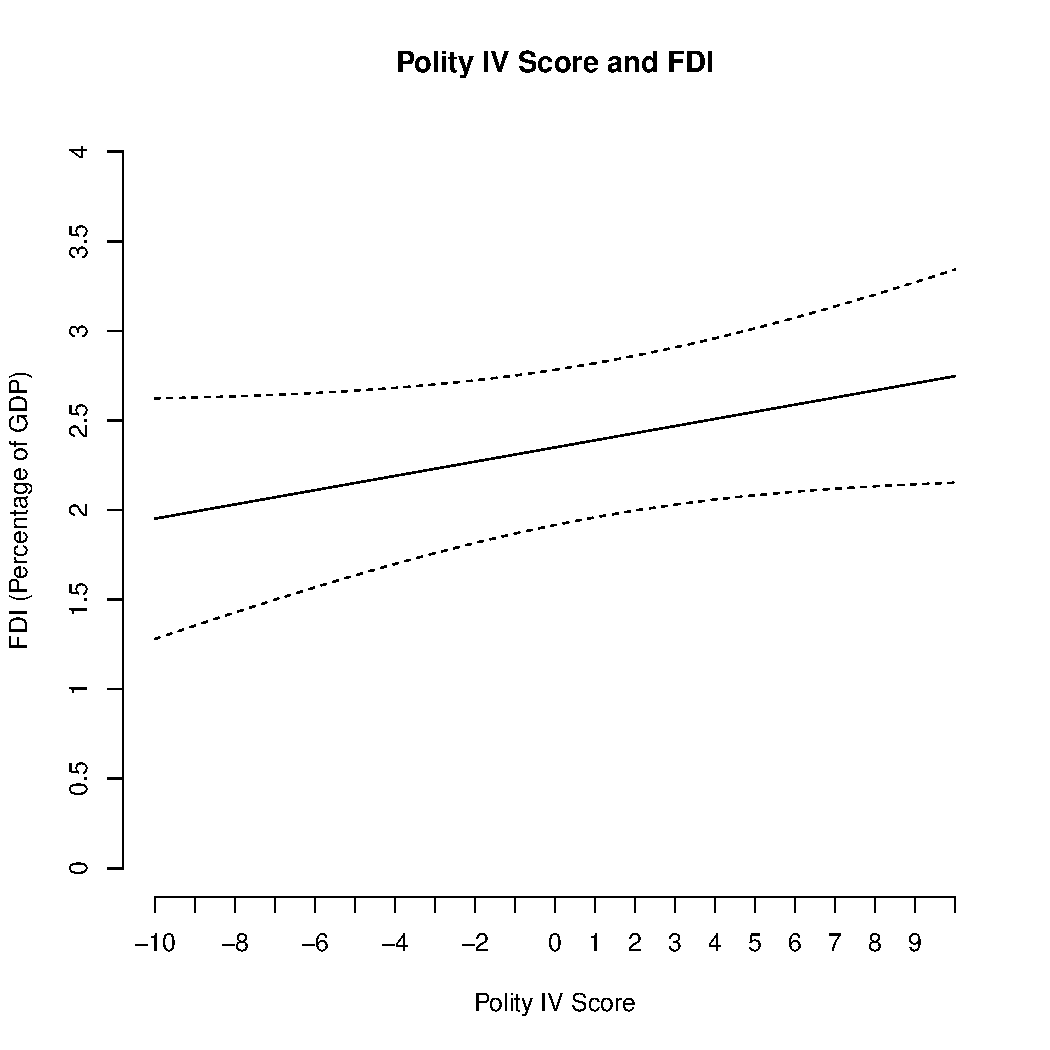
\includegraphics[width=\maxwidth]{figure/unnamed-chunk-3-1} 

\end{knitrout}



\section*{Linear Regression Models Interpretation Questions}

\subsection*{Problem 3}

\paragraph*{a)} If we do not include polynomials of higher order, OLS regression can adequately model only \textbf{linear} relationships between one dependent variable (response variable) and multiple independent variables (predictor variables). The reason for why we can only model linear relationships is that our model assumes that for every independent variable there is only a single slope coefficient that is constant for all values of that independent variable. Polynomials of higher order would allow us to have different slopes at different values of the independent variable.

\paragraph*{b)} OLS regression does not per se tell us anything about causality. OLS regression primarily measures linear relationships between two variables and can give us an answer to the question how to variables are correlated with each other. However, without a strong theory, OLS does not allow us to make statements regarding causality.

There are several reasons for this. First, there could be reverse causality, meaning that the response variable in our model has a causal effect on the predictor variable. Second, there could be endogeneity, meaning that there is mutual causal influence of response and predictor variables. Finally, there could be omitted variable bias, meaning that a third variable influences both the predictor and the response variable. These are the three main reasons why we should not per se view the results of a linear regression as reflecting causality.

\paragraph*{c)} The Residual Sum of Squares (RSS) can be found through the following calculation involving the Root Mean Squared Error (RMSE):

\bigskip

RSS = $(RMSE^2)*(Degrees\ of \ Freedom)$

\bigskip

Furthermore, once we know the RSS, we can use the fact that $R^2 = 1 - \dfrac{RSS}{TSS}$ to find that:

\bigskip

$\dfrac{1 - R^2}{RSS} = \dfrac{1}{TSS}$ \rightarrow $\dfrac{RSS}{1 - R^2} = TSS$

\bigskip

Once we know both the TSS and the RSS, we can easily calculate the RegSS, since the $RegSS = TSS - RSS$.



\section*{Statistical Theory: Linear Regression Models}

\subsection*{Problem 4}

\subparagraph{a)} The definition of b is $\dfrac{Cov(X,Y)}{Var(X)}$. The definition of b' is $\dfrac{Cov(Y,X)}{Var(Y)}.

The formula for variance is $\dfrac{\sum{(x_i - \bar{x})}}{n-1}$. Assuming that the variables X and Y have two or more different values, their variances are always positive. Therefore, the denominator in both equations is positive.

If the variance is always positive, then the sign of the covariance (+, -, or 0) determines the sign of b and b'. In the following equations, + stands for a positive number, - for a negative number, and 0 for zero.

$b = \dfrac{Cov(X,Y)}{+}$ and $b' = \dfrac{Cov(Y,X)}{+}$

Since $Cov(X,Y) = Cov(Y,X)$, the following is true:

If $Cov(X,Y) > 0$, then $b = \dfrac{+}{+}$ and $b' = \dfrac{+}{+}$, meaning that both are positive.

\bigskip

If $Cov(X,Y) < 0$, then $b = \dfrac{-}{+}$ and $b' = \dfrac{-}{+}$, meaning that both are negative.

\bigskip

If $Cov(X,Y) = 0$, then $b = \dfrac{0}{+}$ and $b' = \dfrac{0}{+}$, meaning that both are zero.

\bigskip

It follows that b and b' always have the same sign.



\subparagraph{b)} The intercepts, a and a', do not always have the same sign as we can show with a simple counter example.

Assume that the variables X and Y have the following values:

\begin{center}
 \begin{tabular}{||c c||} 
 \hline
 X & Y \\ [0.5ex] 
 \hline\hline
 0 & 2 \\ 
 \hline
 1 & 3 \\
 \hline
 2 & 4 \\
 \hline
 3 & 5 \\
  \hline
\end{tabular}
\end{center}

Note that in this case $Y = 2 + X$ and $X = -2 + Y$, so a = 2 and a' = -2. In this case a and a' have different signs, meaning that the statement is not true.



\end{document}
